\chapter{Concepts}
\label{chap:concepts}

\section{User Interface}

\begin{wrapfigure}[12]{R}{0.5\linewidth}
	\caption{\label{fig:ui:tablet}Example placement of the control device}
	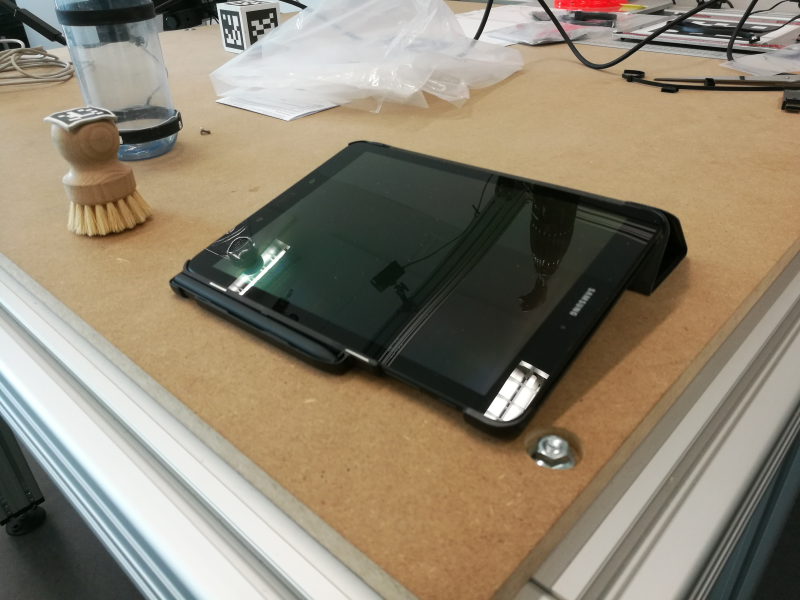
\includegraphics[width=\linewidth]{assets/chpt_concepts/tablet.png}
\end{wrapfigure}

\begin{figure}
	\caption{\label{fig:firstmockup}A first overview of the screen space distribution}
	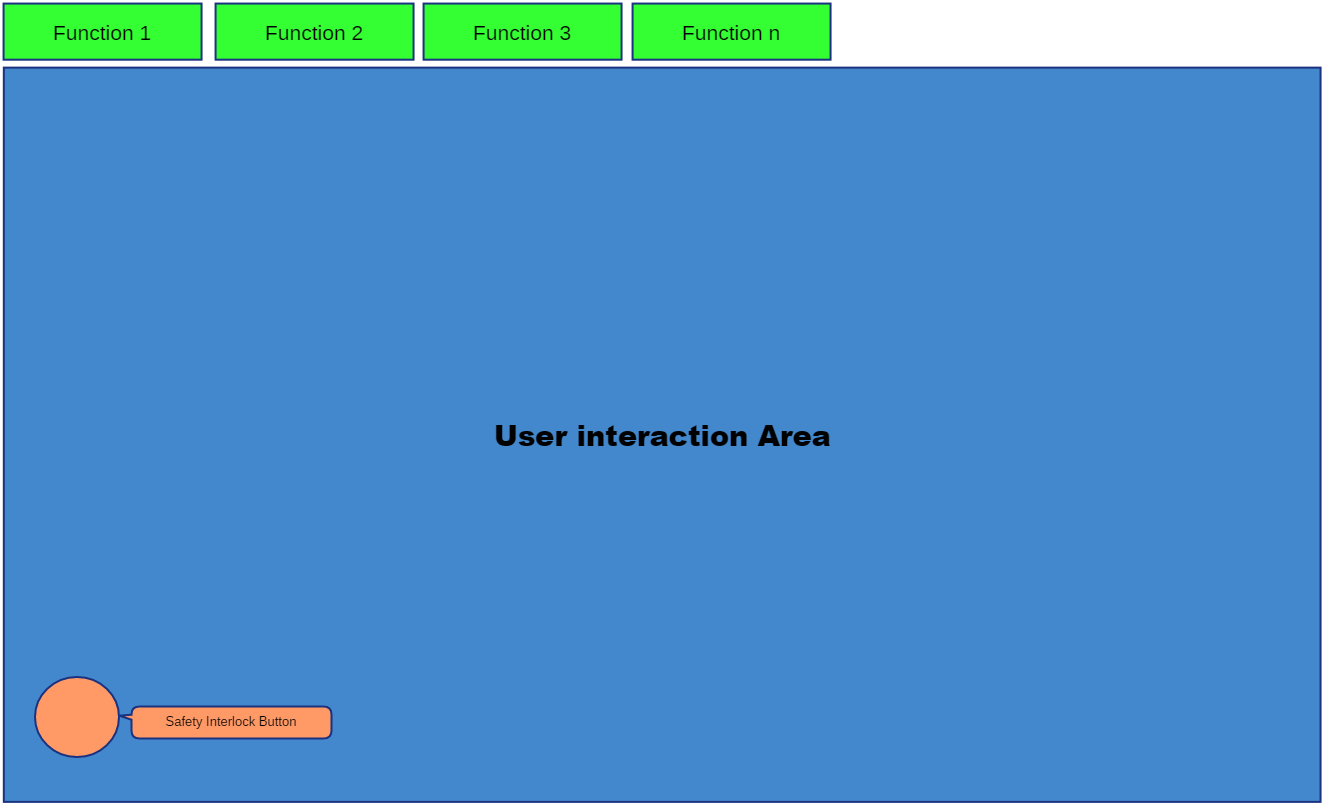
\includegraphics[width=0.9\textwidth]{assets/chpt_concepts/main_touch_interface.png}
\end{figure}

\subsection{Desired position of the Android Tablet}
The application (and thus the screens within it) will be designed for the tablet to be placed in front of the operator on a table. The person should have clear sight on the controlled robot. It seems sensible to place the tablet on the table in front of the robot while looking at it. Most interactions with the application will be performed by touch gestures using the right hand. For better usability a housing or case can be used to position the tablet at a slight angle to the table. 


Interaction with the application is done using the commonly known touch gestures like
\begin{itemize}
	\item Touch (short press on the screen)
	\item Long press (finger remains on a control for a longer period of time)
	\item 1-Finger-Movement
	\item 2-Fingered gestures (\textit{Pinch-Zoom}, Rotation)
	\item 3-Fingered gestures (Rotation, Movement)
\end{itemize}

\subsection{General Screen Layout}
\label{sec:ui:layout}
As a screen of a diagonal size of 10 inches (25.4cm) is very limited compared to the size of the robot's workspace good considerations have to be made according to a well-designed user interface. Since we are mainly operating the robot with touch gestures, significant parts of the screen should be blank, as only few information can be displayed while the user poses his hands above or on the screen. Figure \ref{fig:firstmockup} gives a first overview of how the portions of the screen shall be distributed. The biggest part of the screen is reserved for touch interactions by the user. Since multiple approaches to control the robot shall be implemented, the method shall be selected and switched using a tabbed layout with the tabs on the top, as they use the least space of the screen this way.

\subsubsection{Interlock Button}
On all screens where the robot can be remotely operated, a security interlock button shall be displayed. For the actions on the screen to have effect on the robot (i.e. to be sent to the controller) the button shall remain pressed. This implements the functionality of a dead-man-switch, stopping all robot action once released. Although this is only a software measure it should be a good solution against unwanted movements of the robot as the button can easily be released when pressed with a single finger of the left hand. \textbf{Of course, this software measure does not replace hardware safety measures like emergency switches, but only supports them.}

\subsection{Grasp Synergy Screens}

\begin{wrapfigure}[12]{l}{0.6\textwidth}
	\caption{\label{fig:screen:synergy}Synergy control screen}
	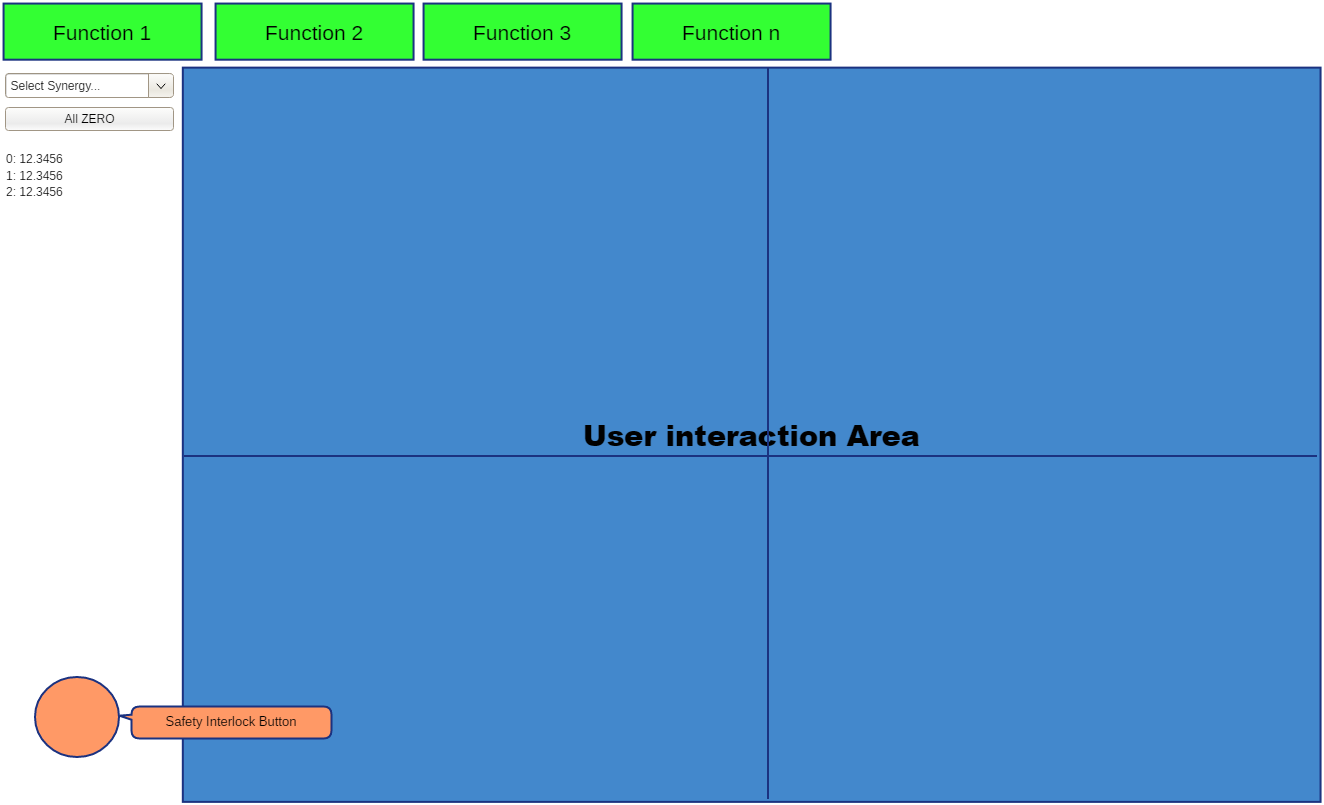
\includegraphics[width=0.6\textwidth]{assets/chpt_concepts/grasp_synergy_page}
\end{wrapfigure}

As the control of grasp synergies allows multiple different types of synergies to be selected, a drop-down selection of the synergy shall be displayed to the left side of the screen. This keeps the right side of the screen clear for better operability by right-hand users. Additionally, a cross of lines shall be displayed on the screen so the user knows where the middle of the touch interaction area is. As described later, this is particularly important in the approach with absolute synergy control (See Chapter \ref{sec:synergies:absolute}). To give the user some information about the state of a synergy, the values of significant amplitudes applied to the synergy shall also be displayed on the left hand side of the screen. A button to set the hand into the synergy's idle state (i.e. all significant amplitudes set to $0$) is also sensible to be implemented. A sample of how this screen could look like is demonstrated in Figure \ref{fig:screen:synergy}.

\subsection{Direct Fingertip Mapping Screen}

As there are no additional controls required to control the direct fingertip mapping, the control screen looks mostly like the general touch interaction screen seen in Figure \ref{fig:firstmockup}.

\subsection{Single Axis/Joint Control}

\begin{wrapfigure}[11]{r}{0.4\textwidth}
	\caption{\label{fig:axiscontrol}Axis control widget with different status indicators}
	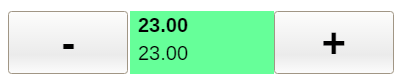
\includegraphics[width=0.4\textwidth]{assets/chpt_concepts/AxisControlGreen}
	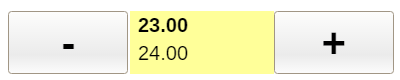
\includegraphics[width=0.4\textwidth]{assets/chpt_concepts/AxisControlYellow}
	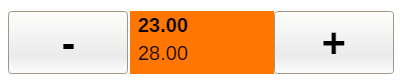
\includegraphics[width=0.4\textwidth]{assets/chpt_concepts/AxisControlRed}
\end{wrapfigure}

An interface shall be implemented to give users the ability to control each joint of the robot individually. This is sensible for a variety of reasons. Firstly, it might sometimes be required to move the robot out of a specific state by moving just one axis and not by applying multiple changes at once. Possible scenarios for this use case could be a state where the robot could harm users or the environment if uncontrolled or unpredictable movements occur. An interface to control joints individually is also very practical for testing purposes, for example if one part of the robot is suspected to be broken.

Within this interface, the currently measured joint angle shall be displayed for each joint, next to the currently set target value (printed in bold). This gives the user a good insight of what state the robot should be in according to the program and what state it actually is in. This shall be supported by a coloured indicator, giving a quick visual feedback on the difference of the target and actual joint angles $\Delta \alpha = |\alpha_{actual} - \alpha_{target}|$. The colours of the visual feedback shall be:

\begin{itemize}
	\item Green for $\Delta\alpha \leq 0.5^\circ$
	\item Yellow for $0.5^\circ < \Delta\alpha \leq 2.5^\circ$
	\item Red for $\Delta\alpha > 2.5^\circ$ 
\end{itemize}

The buttons to move the axis shall be displayed right and left of the angle displays. The visual feedback shall be shown as the background of the angle values. All these requirements put together, an axis control widget for a single joint or axis could look like depicted in Figure \ref{fig:axiscontrol}. To each control widget, a heading will be added to unambiguously denote which axis or joint will be controlled when using the corresponding buttons.

Multiple of these widgets shall be added to the axis control screen, one for each controllable joint or axis. This will result in a screen containing 29 of these (22 for the hand, 7 for the robot arm). To get an idea of how the control screen for individual joint control will look like, the reader is referred to Figure \ref{fig:axiscontrol:screen}\footnote{Please note, however, that the number of hinted joint control widgets does not resemble the actual number of controllable joints for each part of the robot.}. 

\begin{figure}
	\caption{\label{fig:axiscontrol:screen}Axis control screen draft}
	\frame{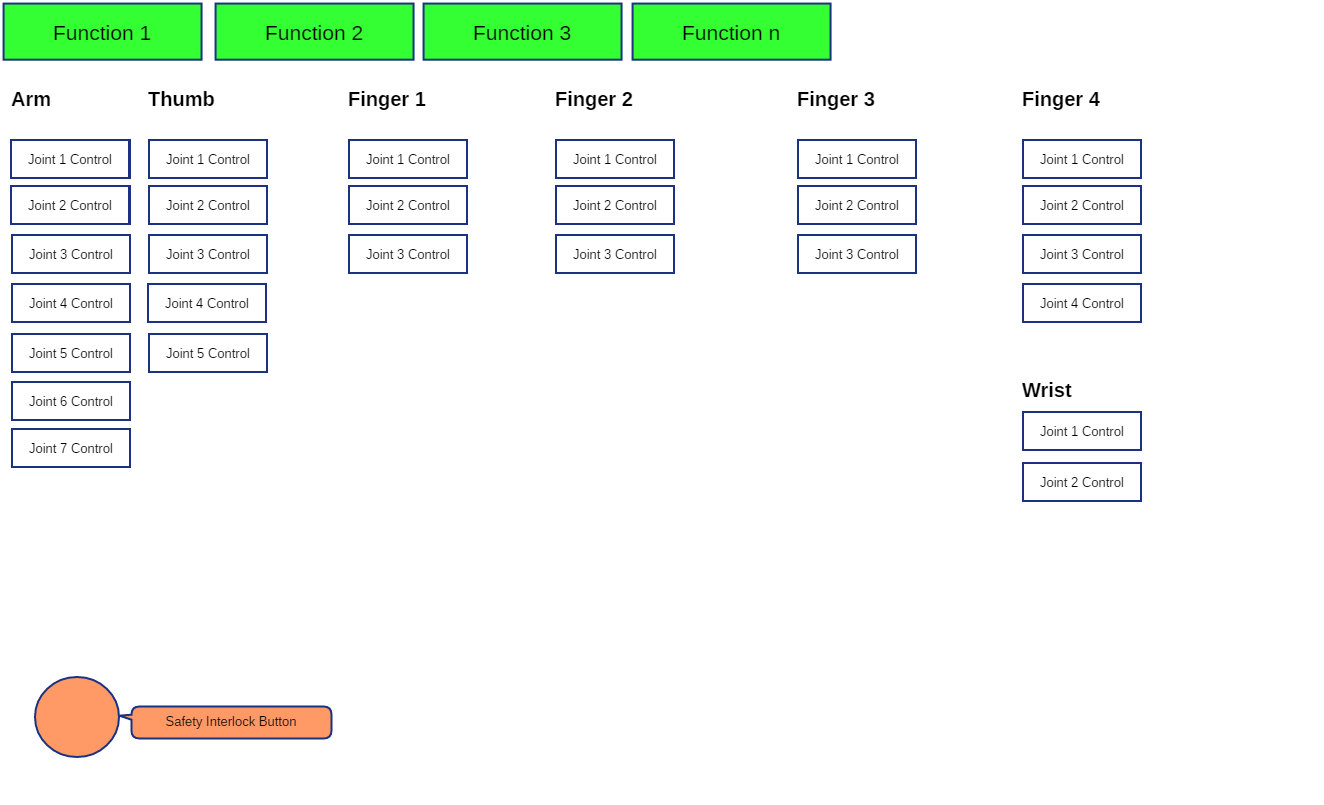
\includegraphics[width=0.8\textwidth]{assets/chpt_concepts/AxisControlPage}}
\end{figure}

\section{Using the BioIK Service}
\label{sec:robotarm:ctrl}

The BioIK serivce (see Section \ref{sec:bioik}) is used according Section \ref{sec:using_services}. The important messages types are:
\begin{itemize}
	\item \textbf{GetIK} The combined Request/Response service message type
	\item \textbf{GetIKRequest} The message type containing the request to the service
	\item \textbf{GetIKResponse} The message type containing the response of the service
	\item \textbf{IKRequest} The actual request data
	\item \textbf{IKResponse} The actual response data
\end{itemize}

In the process of getting joint data from the BioIK service, the message types \textit{IKRequest} and \textit{IKResponse} are most important, because they contain the data needed on both sides. As the used message types contain a large number of members, only those significant for this thesis will be discussed within this section.

The \textit{IKRequest} message contains information about the current robot state and about the desired robot pose (see Table \ref{tab:msg:ikrequest}). The so-called \textit{goals} used here are \textit{PositionGoal}, \textit{OrientationGoal} and \textit{PoseGoal}, which is basically a combination of the first two. All goals contain a link name, which describes the end-effector that shall be brought to the given position or orientation. A \textit{PoseGoal} contains a \textit{Point} message type, which is a vector in 3D space. The \textit{OrientationGoal} consists of a \textit{Quaternion} which encodes the desired orientation of the end-effector in space. Lastly, the \textit{PoseGoal} contains both, a \textit{Point} and a \textit{Quaternion}, defining a distinct position and orientation in space. When provided with the current state of the robot, the IK algorithm begins looking for solutions at this state, possibly speeding up the overall solving process. Different goals for multiple end-effectors (called \textit{links}) can be passed to the BioIK service which will then try to find a solution fulfilling all of the given goals.

When the BioIK service has finished it returns a \textit{IKResponse} (Table \ref{tab:msg:ikresponse}) to the caller. Within the response, a status (or error) code is given, indicating success or failure of the algorithm. If the status code indicates 0 (meaning success), the \textit{RobotState} field of the message contains joint angles for all joints of the robot, representing a state in which the goals passed to the service in the first place are reached. All angles for the joints (in \textit{IKRequest} as well as \textit{IKResponse}) are given in radians.

\begin{table}
	\caption{Important contents of the IKRequest message type\label{tab:msg:ikrequest}}
	\begin{tabularx}{\linewidth}{|l|X|}
		\hline
		\textbf{Field} & \textbf{Description} \\
		\hline
		string group\_name & The MoveGroup name of the robot. Fixed to \textit{lwr\_with\_c5hand} here \\
		\hline
		bool approximate & If true, an approximate solution is returned when no exact solution could be found by the IK solver \\
		\hline
		duration timeout & The timeout after which the solver stops looking for solutions. If no solution was found by then, an approximate solution is returned if approximate is true, otherwise no solution is returned. Fixed to one second here. \\
		\hline
		int32 attempts & Number of attempts the solver shall take. Fixed to 1 here. \\
		\hline
		string[] fixed\_joints & Names of the joints the IK solver shall not move while looking for solutions. \\
		\hline
		bool avoid\_collisions & If true, the BioIK solver tries to find solutions that do not collide with the environment (and the robot itself). \\
		\hline
		RobotState robot\_state & The current state of the robot. Contains a JointState message containing the current joint angles of all joints. These values are taken as a starting point while searching for solutions. \\
		\hline
		PositionGoal[] position\_goals & The positions of multiple end-effectors that shall be reached with the IK solution. \\
		\hline
		PoseGoal[] pose\_goals & The poses of multiple end-effectors that shall be reached with the IK solution. A pose goal is similar to a position goal, but extends it by a desired orientation. \\
		\hline
		OrientationGoal orientation\_goals & The orientations multiple end-effectors shall have within the IK solution. \\
		\hline
	\end{tabularx}
\end{table}

\begin{table}
	\caption{Important contents of the IKResponse message type\label{tab:msg:ikresponse}}
	\begin{tabularx}{\linewidth}{|l|X|}
		\hline
		\textbf{field} & \textbf{Description} \\
		\hline
		MoveItErrorCodes error\_code & An error code stating if a solution was found or not. 0 indicates success, whereas all other values indicate that no solution was found. \\
		\hline
		RobotState solution & If error\_code is 0, this field contains the found solution encoded in a JointState field with an angle for every joint. \\
		\hline
	\end{tabularx}
\end{table}

\section{Grasp Synergies}

In their work \citeauthor{Bernardino2013} describe a way to record hand postures using a data glove and the Shadow C5 robotic hand. The result of their research are data recorded for 8 different grasp postures of the human hand \cite{Bernardino2013}. Using \textit{Principal Component Analysis (PCA)} the datasets for each posture were parametrized. This process resulted in a matrix $S = (s_1, \dots , s_M)$ for each grasp posture with $s_m$ being the eigenvectors of the parametrized grasp postures. For each posture $s_0$ is the mean value of all recorded posture data sets, defining the rest position of the hand within this posture. To get joint angles from these synergy matrices, they have to be multiplied by a vector $\alpha = (\alpha_1, \dots , \alpha_N)$ containing the so-called amplitudes for each parameter. For a given synergy matrix $S$, a synergy offset $s_0$ and amplitude vector $\alpha \in \mathbb{R}^N$, the joint angles $\theta = (\theta_1, \dots , \theta_N)$ are described as
\begin{equation}
\label{eq:syn}
\theta = s_0 + S\alpha
\end{equation}

Since $S$ is sorted in such a way that changes to $\alpha_1, \alpha_2$ and $\alpha_3$ already cover approx. 80-90\% of the variance in the grasp postures recorded\cite{Bernardino2013}, we will only look onto these three amplitudes when implementing the approach to grasping objects in this thesis.

$s_0$ and $S$ are provided by the above research and $\theta_n$ is given in degrees, $\alpha_n$ is $-50 \leq \alpha_n \leq 50$. The goal is to find a good mapping between touch gestures and $\alpha_n$, so that the grasp can be controlled intuitively.

\subsection{Touch Gestures}

To find solutions to map touch gestures to synergy amplitudes, we first generalize the understanding of touch gestures.

\begin{defn}
$p = (p_x, p_y) \in \mathbb{R}^2$ is called a pointer on a touch screen, i.e. the coordinates of a registered finger the user has laid onto the touch surface.
\end{defn}

\begin{defn}
 A set of pointers $G = \{p_1,\dots , p_n\}$ with $|G| \geq 1$ is called a \textbf{gesture}.
\end{defn}

Although pointer positions on a touch screen are usually given in integer numbers, pointers are defined in real space to make the following definitions possible. After having defined gestures, we have a look at different properties of them. Firstly, the two most basic properties of a gesture are defined, being the \textbf{position} and the \textbf{size}.

\begin{defn}
	Let $G$ be a gesture.
	
\begin{itemize}
	\item The \textbf{position} $c(G)$ of G is defined as
	\begin{equation}
	c(G) = \frac{1}{|G|}\sum_{i=1}^{|G|}p_i \qquad  p_i \in G\text{.}
	\end{equation}
	
	\item The \textbf{size} $s(G)$ of G is
	\begin{equation}
	s(G) = \frac{2}{|G|}\sum_{i=1}^{|G|} d(c(G), \quad p_i)
	\end{equation}
	with $p_i \in G$ and $d(x, y) = \sqrt{(y_1 - x_1)^2 + (y_2 - x_2)^2}\quad$ for $x, y \in \mathbb{R}^2$ the euclidean distance between two pointers.
\end{itemize}
\end{defn}

In other words: The position of a gesture is the \textit{center of mass} of all pointers of a gesture. The size is the doubled mean distance of all pointers to the position of a gesture. Before defining the last property of a gesture, the \textbf{orientation} we first have to define what the \textbf{thumb pointer} of a gesture is.

\begin{defn}
	The \textbf{thumb pointer} $th(G)$ of a gesture $G$ is defined as
	\begin{equation}
	th(G) = \left\{
	\begin{array}{ll}
	p_1 & |G| = 1 \\
	p_n \text{ with } p_{n,y} = max\{p_{i,y} : p_i \in G\} & |G| = 2 \\
	p_n \text{ with } d(c(G), p_n) = max\{ d(c(G), p_i) : p_i \in G \}& |G| > 2
	\end{array}
	\right.
	\end{equation}
	
The thumb pointer shall be evaluated and memorized whenever $|G|$ changes, i.e. a pointer is added or removed from a gesture.
\end{defn}

Note that the $y$ coordinate is rising to the bottom, as it is usual on digital screens. Having this in mind the thumb pointer is the lowest pointer in a 2-pointer gesture or the one furthest away from the position of a gesture with 3 or more pointers. The last part of the definition is important, as the lowest pointer does not necessarily remain the lowest when the gesture is rotated on the screen, so to have a consistent definition of the orientation, the thumb pointer may only be evaluated when pointers are added or removed from a gesture.

\begin{defn}
	Let $G$ be a gesture, $b_y = (0, -1) \in \mathbb{R}^2$. For $v = c(G) - th(G)$, the orientation $o(G)$ is defined as
	
\begin{equation}
o(G) = sign(det(b_y\, v)) \cdot acos\left(\frac{v \cdot b_y}{|v| \cdot |b_y|}\right) \, .
\end{equation}	

\end{defn}


In other words the orientation of a gesture is the angle between the vector from the thumb pointer to the position of a gesture and $b_y$, which is pointing upwards in screen coordinates as, again, $y$ is growing downwards. If the determinant of $(v\,b_y)$ is negative, the angle between $b_y$ to $v$ is counter-clockwise\cite{Bronstein2012}. Using this, the values of $o(G)$ range from $-\pi$ (which is $180^\circ counterclockwise$) and $\pi$. 

\subsubsection{Example}

\begin{figure}
	\caption{\label{fig:touch:expl}Example gesture with 3 pointers}
	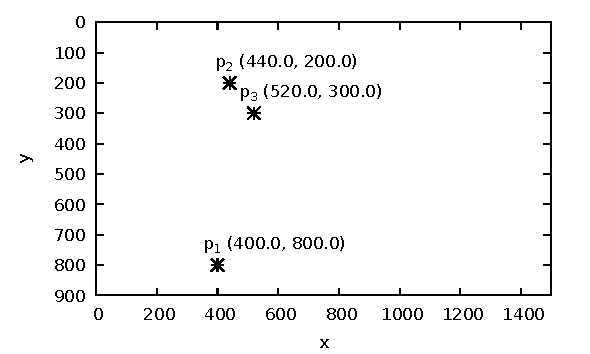
\includegraphics{assets/chpt_concepts/gestures/3pointers_blank.pdf}
\end{figure}

The above definitions will be briefly elaborated with an example of a gesture with 3 pointers. Figure \ref{fig:touch:expl} shows the example gesture. First, the position of the gesture is calculated:

\begin{equation*}
c(G) = \frac{1}{3}\left( \vectwo{400}{800} + \vectwo{440}{200} + \vectwo{520}{300} \right) \approx \vectwo{453.3}{433.2}
\end{equation*}

The size of the gesture is

\begin{align*}
s(G) &= \frac{2}{3}\left( d(c(G), p_1) + d(c(G), p_2) + d(c(G), p_3) \right) \\
&= \frac{2}{3}\left( \left|c(G) - p_1\right| + \left| c(G) - p_2 \right| + \left| c(G) - p_3 \right| \right) \\
&= \frac{2}{3}\left( \left| \vectwo{53.3}{-376.8} \right| + \left| \vectwo{13.3}{233.2} \right| + \left| \vectwo{-66.7}{133.2} \right| \right)	\\
&\approx \frac{2}{3}\left( 380.6 + 233.6 + 147 \right)\\
&\approx 508.8
\end{align*}

Figure \ref{fig:touch:expl_res} shows the example gesture extended with the position of the gesture and a circle with the diameter of the gesture size around the position of the gesture. From the above calculation it can be seen that $p_1$ has the biggest distance to the position of the gesture, that implicates $th(G) = p_1$ as $G$ has more than 2 pointers. With this we can calculate the orientation of the gesture as follows.

\begin{align*}
o(G) &= acos\left( \frac{\vectwo{53.3}{-376.8} \cdot \vectwo{0}{-1}}{380.6 \cdot 1} \right) = acos\left( \frac{376.8}{380.6} \right) \\
&\approx acos\left( 0.99002 \right) \\
&\approx 0.141398 \widehat{\approx} 8.101 ^\circ
\end{align*}

$G$ has an angle relative to the $y$ axis from about $8.1^\circ$.

\begin{figure}
	\caption{\label{fig:touch:expl_res}Example gesture with center and size}
	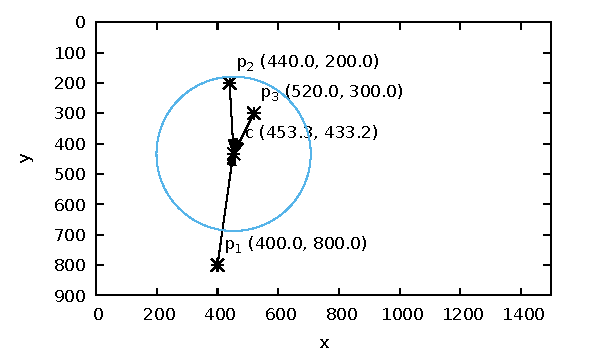
\includegraphics{assets/chpt_concepts/gestures/3pointers_center.pdf}
\end{figure}

\subsection{Absolute Approach}
\label{sec:synergies:absolute}

Within the absolute approach a solution shall be found to map the properties of one or more gestures to the different degrees of freedom of the hand synergy and the arm. To control the hand synergy, it is sensible to control all three significant amplitudes with just one gesture, so the user does not have to change the pointer count of the gesture while operating the hand. This is especially useful as it seems relatively difficult to position the fingers at the exact same place after hacing used another gesture. However, to reproduce a distinct position the pointers have to be placed at the exact same place on the screen.

It is $c:G\rightarrow\mathbb{R}^2$, $s:G\rightarrow\mathbb{R}$ and $o:G\rightarrow\mathbb{R}$, which means if both components of the position are viewed separately it is possible to control as many as four DOF with just one gesture. As, for the hand posture synergies, we only want to control 3 DOF, considerations should be made which properties shall be taken into account for controlling the synergies. It seems best to choose those properties having the biggest range in value:
\begin{itemize}
	\item The $y$ component of the gesture position has a range of slightly less than the screen height
	\item The $x$ component of the gesture position has a range of slightly less than the screen width
	\item The orientation has a range of $2\pi$.
	\item The gesture size has a range corresponding to the user's finger span, which should usually be around $\frac{2}{3}$ of the screen width
\end{itemize}

In first tests, it turned out complicated to have the position of a gesture remain at the same place in both axes while rotating it or changing its size, the $x$ component of the position is chosen as one DOF, since it is larger and thus it is possible to have more granular control on the amplitude's value.

All mappings from gestures' properties to DOF values shall be done linearly. A general approach has to be found to create these linear functions for all DOF of the hand synergy as well as the arm.

\subsubsection{Linear DOF mapping}

There are multiple requirements for the function to find. Firstly, the linear equation shall be defined by two points $x, y \in \mathbb{R}^2$ with $x_1$ and $y_1$ being in gesture property's space and $x_2$, $y_2$ being in the corresponding DOF space (amplitude or arm position). Secondly, the output value shall be limited to the possible values of the DOF, for the synergies' amplitudes this will be $-50$ and $50$.

A function $lm:(x \in \mathbb{R}^2, y \in \mathbb{R}^2, v_{min} \in \mathbb{R}, v_{max} \in \mathbb{R}, p \in \mathbb{R}) \rightarrow \mathbb{R}$ shall be found with the parameters being the two points the linear equation spans in between, the minimum and maximum output value and the value of the gesture property. It outputs the value that can then directly be passed into the DOF value.

Finding the linear equation spanned between two points $x, y \in \mathbb{R}^2$ is relatively easy. Beginning from the general linear equation
\begin{equation*}
f(x) = m \cdot x + b
\end{equation*}
it is well known that

\begin{align*}
m &= \frac{y_2 - x_2}{y_1 - x_1} \\
b &= x_2 - m \cdot x_1  \\
&= x_2 - \frac{y_2 - x_2}{y_1 - x_1} \cdot x_1
\end{align*}

To clip a value $v$ to a minimum and maximum value $v_{min}$ and $v_{max}$ (with $v_{min} \leq v_{max}$) one $min$ and a $max$ operation have to be performed\footnote{If it's unknown which limiting value is greater, two $min$ and $max$ operations have to be performed: $clip(v_1, v_2, v) = max(min(v_1, v_2), min(v, max(v_1, v_2)))$}:

\begin{equation*}
clip(v_{min}, v_{max}, v) = max(v_{min}, min(v, v_{max}))
\end{equation*}

Combination of the linear equation and the $clip$ function results in the function defined below.

\begin{defn} Let $lm : (\mathbb{R}^2, \mathbb{R}^2, \mathbb{R}, \mathbb{R}, \mathbb{R}) \rightarrow \mathbb{R}$ a function for \textbf{linearly mapping} a value $p$ onto a linear function between two points $x, y \in \mathbb{R}^2$ with the output limited between $v_{min}, v_{max} \in \mathbb{R}$. Then $lm$ is
\begin{equation}
\label{eq:lm}
lm(x, y, v_{min}, v_{max}, p) = clip\left(v_{min}, v_{max}, \left( p \cdot \frac{y_2 - x_2}{y_1 - x_1} + x_2 - \frac{y_2 - x_2}{y_1 - x_1} \cdot x_1 \right)\right) \, .
\end{equation}
\end{defn}


\subsubsection{Mappings}

Let $w_{screen}$ be the width of the screen in pixels, $\alpha \in \mathbb{R}^N$ the vector of amplitudes for a selected synergy $S$, $G$ a gesture with $|G| = 2$. The proposed mappings for later implementation are:
\begin{itemize}
	\item $\alpha_1 = lm\left((1200, 50), (300, -50), -50, 50, s(G)\right)$
	
	As the size of a gesture is the property easiest to manipulate (with 2 pointers by the so-called pinch-zoom-movement) the amplitude with the biggest effect is assigned to it. The values of 1200 and 300 are chosen as 1200 is the size of a gesture with normally spanned fingers, 300 is the size of a gesture when the pointers are already relatively close. Values lower than 300 render the amplitude value of $-50$ of being unreachable, as pointers are perhaps not be able to be placed that close.
	
	\item $\alpha_2 = lm\left((w_{screen} \cdot 0.25, 50), (w_{screen} \cdot 0.75, -50), -50, 50, (c(G))_1\right)$
	
	For the second significant amplitude the $x$ component of the gesture position is chosen. It is mapped between $\frac{1}{4}$ and $\frac{3}{4}$ of the screen's width as the actual limits cannot be reached with gesture positions due to all pointers having to be at this border then.
	
	\item $\alpha_3 = lm\left( \left( -\frac{\pi}{2}, 50 \right), \left( \frac{\pi}{2}, -50 \right), -50, 50, o(G) \right)$
	
	For the third significant amplitude the orientation is mapped from $-90^\circ \widehat{=} -\frac{\pi}{2}$ to $90^\circ \widehat{=} \frac{\pi}{2}$. Rotations to values greater or less than these have shown to be only possible when moving the tablet or changing the gesture's size and position.
\end{itemize}

$\alpha_{1,2,3}$ are evaluated simultaneously whenever a pointer's position within the gesture changes. Joint angle values are then calculated using (\ref{eq:syn}) with $S$ being the currently selected synergy. Once the joint values are calculated they can be published to the ROS nodes of the Shadow C5 hand.

\subsection{Relative Approach}
\label{sec:app:rel}
Within the relative approach, the values of the significant amplitudes shall not depend on the actual properties of a gesture but on the change each property experiences. This makes it necessary to store the current value of the amplitudes and initialize them, e.g. with 0. Whenever a gesture changes, the difference of the properties is evaluated and mapped to a difference of the amplitude which is then applied.

\begin{defn}
Let $G$ be a gesture. $G(t)$ describes the state of the gesture (i.e. the position of the pointers within the gesture) at time $t$. Then
\begin{equation}
c_i(G) = c(G(t_0 + i \cdot \Delta t)) \, .
\end{equation}
Accordingly, $s_i(G)$ and $o_i(G)$ are defined.
\end{defn}

\begin{defn}
Let $G$ be a gesture. At the time $i$ it is
\begin{equation}
\Delta c(G) = c_i(G) - c_{i - 1}(G) \, .
\end{equation}
Again, $\Delta s(G)$ and $\Delta o(G)$ are defined accordingly.
\end{defn}

With the above definitions we can describe the change of $G$ between two time steps and the change of the gesture's properties between two time steps. The touch pointers are evaluated by the Android operating system periodically, so while a touch pointer is present on the screen, periodic updates are sent to the application. As we do not know the time steps, $\Delta t$ may be small, in particular it may be $0$ without affecting the following calculations.

Next, a rate of change of the output value has to be declared. This rate is given in $\frac{\text{value change}}{\text{property change}}$. If, for example, the value of an amplitude shall change by $c_v = 25$ every $c_p = 1000$ pixels the gesture is moved in one direction, the value would be $\frac{c_v}{c_p} = \frac{25}{1000} = 0.025$. For reasons of simplicity, $c_v$ and $c_p$ shall be passed to the relative change function defined below.

\begin{defn}
Let $rm : (\mathbb{R}, \mathbb{R}, \mathbb{R}, \mathbb{R}, \mathbb{R}, \mathbb{R}) \rightarrow \mathbb{R}$ be the \textbf{relative mapping} function that alters the value $v_{old}$ by the changed parameter $\Delta p$ at the rate of change $\frac{c_v}{c_p}$ while clipping the output between $v_{min}$ and $v_{max}$ with $v_{min} \leq v_{max}$. Then

\begin{equation}
rm(c_v, c_p, v_{min}, v_{max}, v_{old}, \Delta p) = clip(v_{min}, v_{max}, v_{old} + \frac{c_v}{c_p} \cdot \Delta p) \, .
\end{equation}
\end{defn}

Updating the output value upon a changing gesture takes two steps, for example with amplitude $\alpha_1$:
\begin{align*}
\alpha_{1,new} &= rm(50, 1200, -50, 50, \alpha_1, \Delta s(G)) \\
\alpha_1 &= \alpha_{1,new}
\end{align*}

For $\alpha_2$ and $\alpha_3$ the calls to $rm$ are accordingly:
\begin{align*}
\alpha_{2,new} &= rm(50, 1200, -50, 50, \alpha_2, (\Delta c(G))_1) \\
\alpha_{3,new} &= rm(40, \pi, -50, 50, \alpha_3, \Delta o(G))
\end{align*}

Whether these values are well chosen and usable has to be evaluated during tests. When all amplitudes have been calculated the process of calculating the joint angles and publishing them is the same as in Section \ref{sec:synergies:absolute}.

\subsection{Arm Control}

\begin{wrapfigure}{R}{0.5\linewidth}
\caption{\label{fig:arm:coord}The coordinate system relative to the arm}
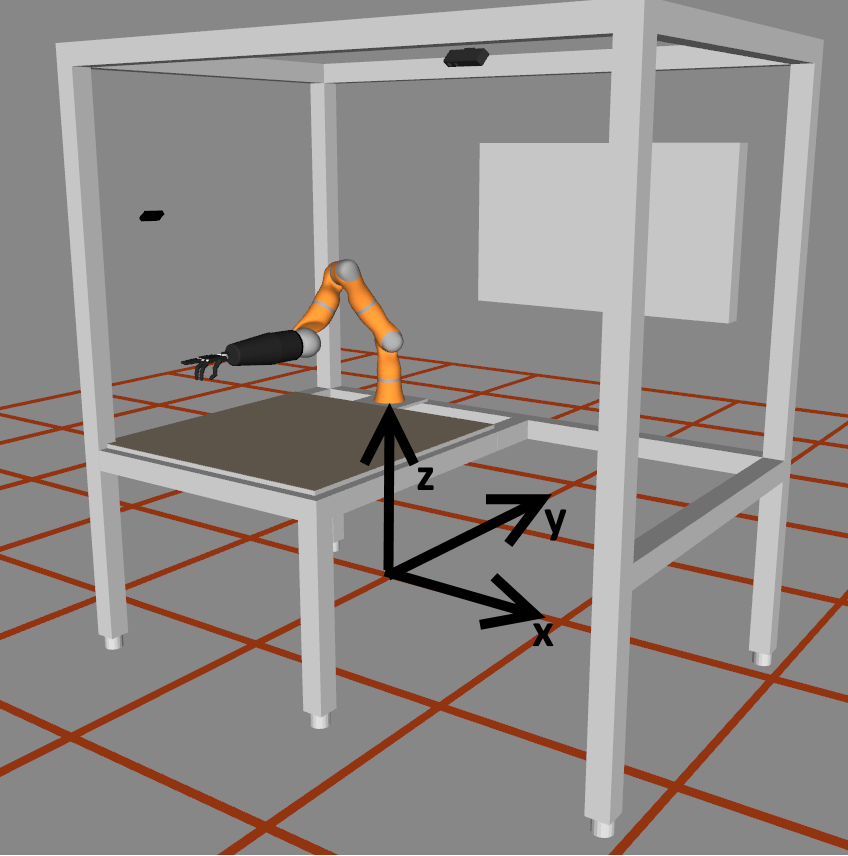
\includegraphics[width=\linewidth]{assets/chpt_concepts/coordinates.png}
\end{wrapfigure}

Controlling the arm with touch gestures is not as easy as controlling the grasp synergies since the arm's joint angles have to be calculated using the BioIK service. The objective is to give the user the opportunity to control the position of the robot hand's palm in Cartesian coordinates. To achieve this, it is important to know the orientation of the coordinate system around the arm as well as \textit{safe} coordinates, where the robot arm can move without causing any danger to its environment. Having a look at Figure \ref{fig:arm:coord} gives a good insight in the coordinate system used. Potentially, an arbitrary coordinate system could be used, but the BioIK service at the point of writing only accepts coordinates in the so-called \textit{world} coordinate system. It has its origin on the floor below the robot arm's base. Each square in the illustration represents one meter in the real set-up. The shown model is assumed to be sufficiently exact to use it as a simulation for the real robot with its surroundings. It is important to keep in mind that the y coordinate is counter-intuitively rising to the back, which means it is falling in the direction to the front. Also, from the robot's perspective, the x axis is oriented to the left.

\begin{wraptable}{L}{0.3\linewidth}
	\caption{\label{tab:safeaxes}Position limits for the robot's hand's palm}
	\begin{tabular}{|c|c|c|}
		\hline
		\textbf{Axis} & \textbf{Min.} & \textbf{Max.} \\
		\hline
		x & $-0.2$ & $0.4$ \\
		\hline
		y & $-1.2$ & $-0.8$ \\
		\hline
		z & $1.05$ & $1.17$ \\
		\hline
	\end{tabular}
\end{wraptable}

In order to prevent damages to the robot or its environment, a \textit{bounding box} has to be found where the robot's movements do not cause any unwanted movements. Unwanted movements can occur since the shortest way from position $x$ to position $y$ may be very short in cartesian space, but still very long in joint coordinates. It is important to keep in mind, that for very close points, the BioIK service might output very different joint positions, as it assumes the new solution more fitting than the old one. This, however, results in a quite small work space for the robot compared to the overall table size. For the first approach, the limits for all 3 axes assumed \textit{safe} are denoted in Table \ref{tab:safeaxes}.

To map touch interactions to positions of the hand's palm the same functions as in Sections \ref{sec:synergies:absolute} and \ref{sec:app:rel} are used with the clipping borders set to the safe axes' limits. As a starting point, the x axis is mapped to the x position of a three-pointer gesture, the z axis to the y position of a three-pointer gesture. As before, only half of each screen dimension will be mapped, leaving out a quarter on each end to make it easier to reach all limits. The y axis will later be mapped to another property of the three-pointer gesture or the position of a four-pointer gesture. Once the desired palm position was calculated it is passed to the BioIK service first, the resulting joint angles returned by the service are then passed to the robot.

\section{Direct Fingertip Mapping}

As \citeauthor{conf:humanoids:TohHLBZP12} state in their work, dexterous grasping and telemanipulation tasks frequently focus on precise control of fingertips in a plane surface\cite{conf:humanoids:TohHLBZP12}. They directly map fingertip positions from the touchscreen to a plane in the working space. As this approach seems interesting it shall also be implemented within this thesis as a third approach.

In this approach heavy use of the BioIK service is made, as not only the position of the hand's palm will be given to the service as a goal, but potentially up to 5 positions for each fingertip will be passed. For the first approach only 3 fingertips shall be usable by the functionality. To find out which positions in three-dimensional space shall be passed for the fingertips, we first have to define a plane the fingertips shall be placed on in three-dimensional space. This is done using the parametrized form to represent a plane 

\begin{equation*}
\vec{E} = \vec{b} + t\cdot \vec{e_1} + s \cdot \vec{e_2}
\end{equation*}

with $\vec{b}$ being the base vector of the plane and $\vec{e_1}$, $\vec{e_2}$ determining the orientation of the plane from the base. It is $|\vec{e_1}| = |\vec{e_2}| = 1$ and $\vec{e_1} \cdot \vec{e_2} = 0$, which means that on the surface a new two-dimensional coordinate system is \textit{created} with its origin in $\vec{b}$. By assigning the $x$ and $y$ coordinates of a point to $t$ and $s$, points from a two-dimensional coordinate system can then easily be mapped into three dimensions.

As one unit in the robot's coordinate system represents one meter in the real world, the coordinates of pointers on the screen shall be calculated in meters of distance to the screen's origin (which usually is the top-left corner). The position of a pointer is known in pixels and the screen resolution is known in dots per inch (DPI). To transform a pixel value $p$ into meters on a screen with a resolution of $r$ DPI, the calculation
\begin{equation*}
p_m = \frac{p}{r} \cdot \frac{2.54}{100}
\end{equation*}
has to be made, as an inch ($in$) is $2.54cm$. The resulting values can then be passed into the equation for the surface to get the corresponding points in the higher dimensional space. These points have to be calculated for each fingertip on the screen, the resulting positions shall then be sent to the BioIK service, resulting in joint angles for every joint on the robot to reach these positions.

To tilt the plane the fingertips are placed on the only things that have to be changes are the vectors $\vec{e_1}$ and $\vec{e_2}$ to span a surface which has another orientation. Also, to move the fingertips in space (e.g. to drag an object in one place and put it to another) no more work has to be done than changing $\vec{b}$. 

For first tests, the vectors defining the plane are chosen as follows:
\begin{itemize}
	\item $\vec{b} = \vecthr{0.1}{-1.1}{1.2}$
	
	This value is relatively straight ahead of the arm and about 15-20cm above the table. This point represents the top-left corner of the touchscreen. Fingertips are mapped using this point as a base in the coordinate system where one unit is one meter. This following two spanning vectors are chosen accordingly.
	\item $\vec{e_1} = \vecthr{-1}{0}{0}$
	\item $\vec{e_2} = \vecthr{0}{1}{0}$
\end{itemize}

The x value rises to the left for the robot's coordinate system, but to the right for the tablet'S screen, which is why the first component of $\vec{e_1}$ is negative. The robot's coordinate system's $y$ coordinate rises to the bottom, so does the $y$ coordinate of the touch screen, the corresponding component in $\vec{e_2}$ is therefore positive (See Figure \ref{fig:dfmt:coords} for a visual comparison of the coordinate systems).

\begin{figure}
	\caption{\label{fig:dfmt:coords}Comparison of the coordinate systems between which shall be mapped. Left: Tablet, Right: Arm coordinate system}
	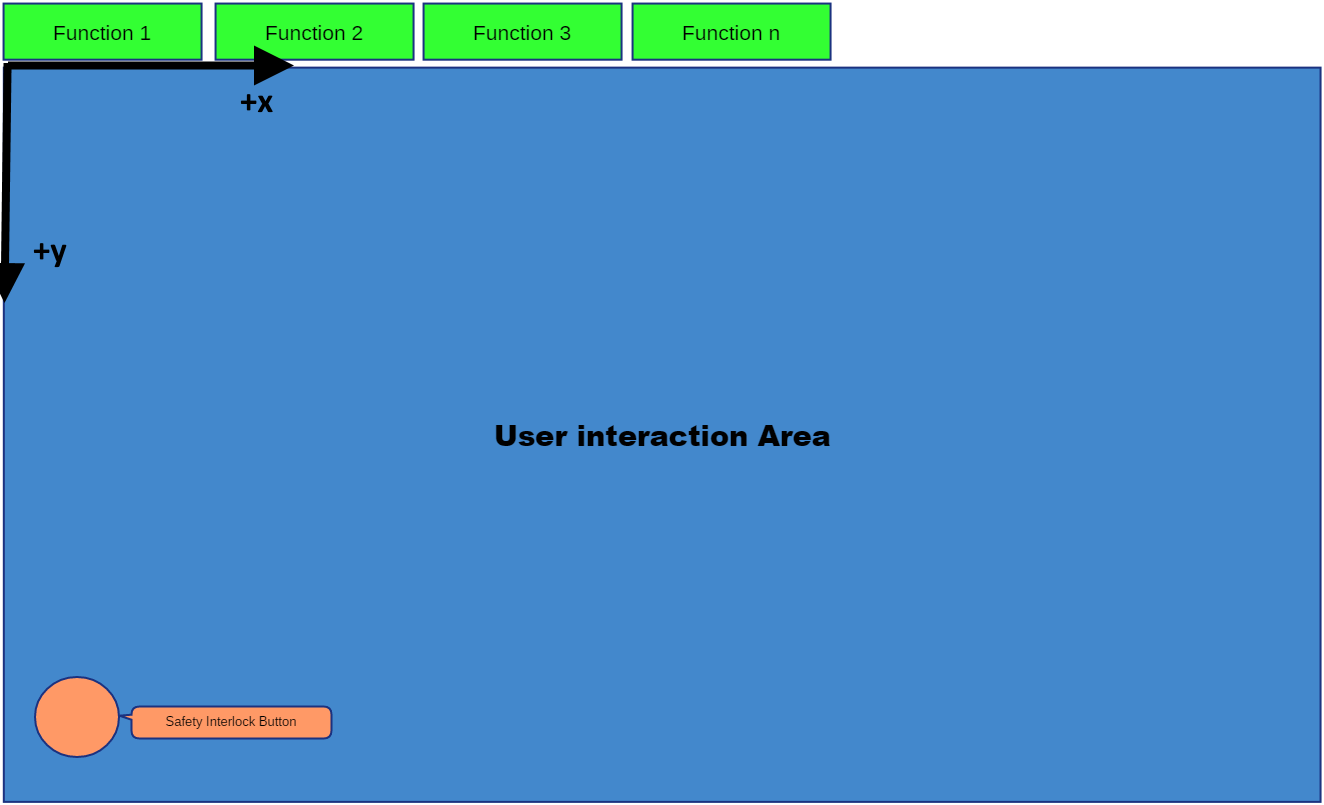
\includegraphics[width=0.6\linewidth]{assets/chpt_concepts/dfmt_coord_screen.png}
	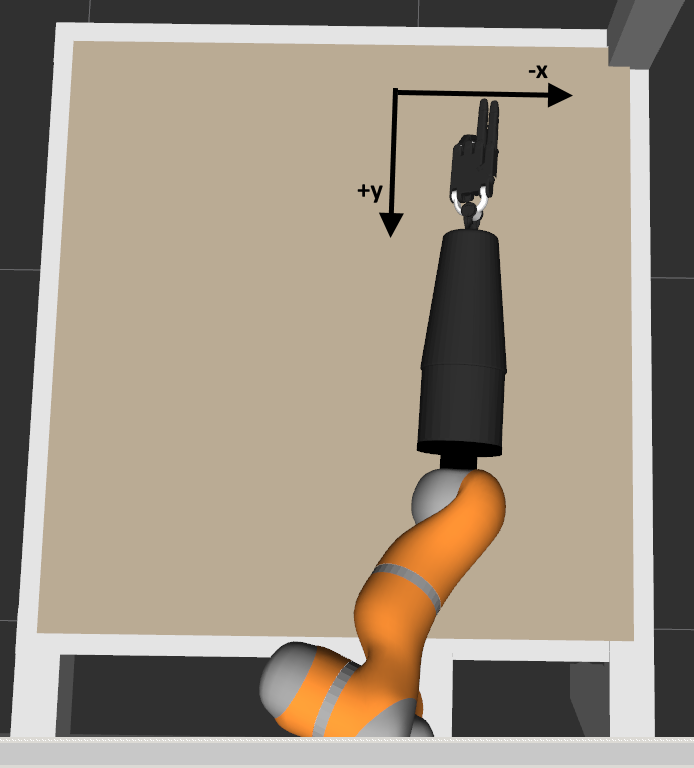
\includegraphics[width=0.4\linewidth]{assets/chpt_concepts/dfmt_coord_arm.png}
\end{figure}

\section{Software Architecture}

Within this section the software architectural design will be discussed. The goal is to create a software design which is easily extensible by further work, making the software a basis for future research. To accomplish this, use of well-known design patterns is made. The three most commonly used patterns in the software are:
\begin{itemize}
	\item Model-View-Controller (MVC)
	\item Observer
	\item Singleton
\end{itemize}

The use of all three is described by examples from the overall software design. \citeauthor{Eilebrecht2013} give a good overview over existing patterns and their use-cases and implementation in \citetitle{Eilebrecht2013}\cite{Eilebrecht2013}, which is where the information about patterns used in the following sections was mainly taken from.

\subsection{Model-View-Controller (MVC)}

\begin{figure}
	\caption{\label{fig:conc:mvc}General Model-View-Controller separation}
	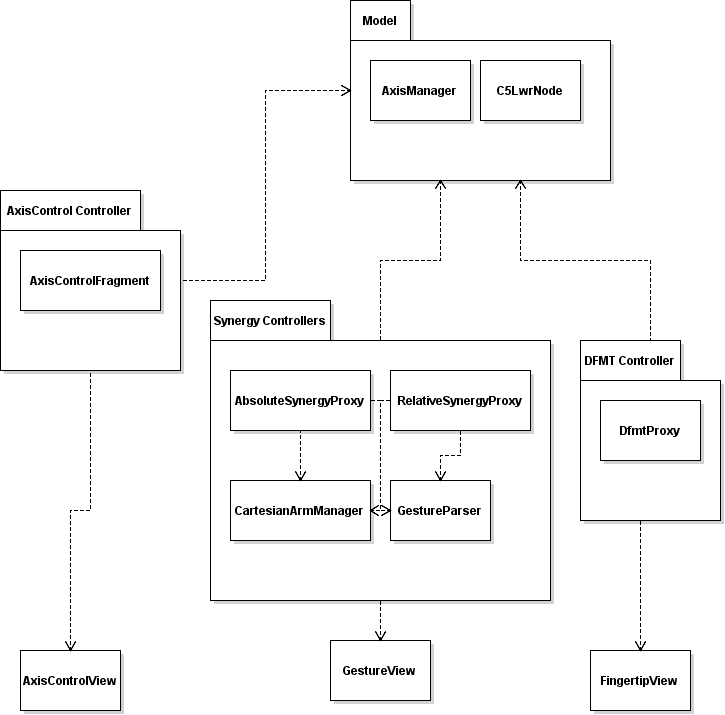
\includegraphics[width=\linewidth]{assets/chpt_concepts/sw/mvc.png}
\end{figure}

Model-View-Controller is a pattern widely used in applications where a set of data (e.g. data from a database) shall be displayed and modified from within multiple interfaces (so-called views)\cite{Eilebrecht2013}. To accomplish this, a \textit{Controller} is set in between the data (\textit{Model}) and the interface implementation (\textit{View}). This \textit{separation of concerns} makes it easy to extend or replace one of the three modules without directly affecting the others. A controller gets data from the \textit{Model}, prepares it for display and passes it on to the \textit{View}, where the concrete display of the data is then defined. The Controller gets feedback from the view, which may then be converted into actions affecting the Model again. Within the developed app design, all three modules can be found, although not always a single class can be assigned for one module. Figure \ref{fig:conc:mvc} gives a rough overview of how the different functionalities are distributed between classes.

\subsubsection{Model}

The Model, which in this case is the data about the robot and its joints, is accessed using the \textit{AxisManager}. The actual communication is done within the \textit{C5LwrNode} class, encapsulating all ROS-specific calls and hiding away the actual communication layer from the rest of the application. Having chosen this design it is relatively easy to replace either the joint data management or the communication layer to the robot.

The \textit{AxisManager} offers functionality to get or set information for each axis of the robot. It gives interface methods to
\begin{itemize}
	\item Get or set the current angle
	\item Enable or disable continuous movement
\end{itemize}
of each joint. It is lockable, meaning that - when locked - no axis updates are accepted by callers, stopping all movements of the robot independent from other controllers. This functionality is important for the safety interlock button described in Section \ref{sec:ui:layout}.

Angle representation within the \textit{AxisManager} is in degrees, whereas the communication with ROS takes place in radians. Conversion between those two has to be made in all actions. To make this conversion functionality exchangable, an interface is declared called \textit{ValueConverter}, allowing to define and assign each joint a different converter. The only implementation used in this application, however, is the \textit{AngleRadianConverter}, converting angles from degrees to radians and vice versa.

The \textit{C5LwrNode} class is a \textit{rosjava} node offering all ROS-specific interfaces to the application. Joint angles are received by the node and passed to the \textit{AxisManager} over an implementation of the \textit{Observer-Pattern} (see Section XY). It also receives joint angles over the observer pattern (by \textit{AxisManager}), passing them on to the robot over ROS. Additionally the BioIK service calls are implemented within the node. This on the one hand creates the need for controller classes to call more than only the \textit{AxisManager}, but encapsulates all ROS specific calls to one class, which was assumed as the smaller drawback here. The conglomerate of \textit{AxisManager}, \textit{C5LwrNode} and all helper classes represents the \textit{Model} within the software design.

\subsubsection{View}

The \textit{View} modules are represented by classes implementing the \textit{View} class from android. They display data either directly from the \textit{AxisManager}, like the axis control page (\textit{AxisControlFragment}) or states of e.g. touch gestures, like \textit{GestureView}, which is used in the pages implementing the grasp synergy control functionality. The type of display is very different, specific implementations are described in section \ref{sec:impl:ui} in a more detailed manner.

As the most important feedback to the user should be the action of the operated robot itself, the view modules are not as elaborated and specifically designed as the other two. As seen in Figure \ref{fig:conc:mvc}, the view usually consists of a single class, whereas \textit{Model} and \textit{Controller} are deeper partitioned and described.

\subsubsection{Controller}

Multiple types of controllers exist in the application. There are controllers that take gestures as an input and provide joint angles as an output (\textit{SynergyProxies}, \textit{AbsoluteSynergyProxy} and \textit{RelativeSynergyProxy} for absolute and relative synergy control) and ones that take gestures as an input and output joint angles for the arm, but by using the ROS functionality offered by the \textit{C5LwrNode} (\textit{CartesianArmManager}). As these classes are coupled relatively strong, they can be seen as one controller divided into multiple sub-controllers. Also, the touch parsing functionality used by both synergy approaches is encapsulated into its own class (\textit{GestureParsing}), taking touch input data from the \textit{View} and outputting gesture information.

For the direct fingertip mapping approach, the number of classes is small compared to the other approaches. The \textit{DfmtProxy} takes care of parsing the touch data provided by its corresponding View (\textit{FingertipView}), requesting joint angles from the \textit{C5LwrNode} and passing them on to the \textit{AxisManager}.

\subsection{Observer}

\begin{wrapfigure}[13]{L}{0.5\linewidth}
	\caption{\label{fig:conc:obs1}Observer-Pattern for GestureParser}
	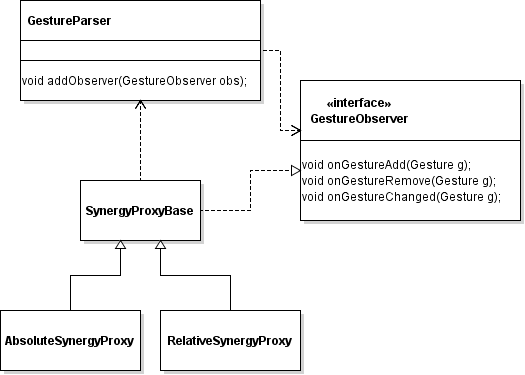
\includegraphics[width=\linewidth]{assets/chpt_concepts/sw/gesture_observer.png}
\end{wrapfigure}

Multiple classes have to exchange data between each other and have to be able to report data changes at arbitrary times. To prevent the occurrence of circular dependencies between classes a variation of the \textit{Observer-Pattern} is used within the application. The \textit{Observer-Pattern} is used to give loosely coupled classes the ability to unidirectionally give notifications to each other about data changes\cite{Eilebrecht2013}.

There are two main uses of the \textit{Observer-Pattern}: 
\textit{SynergyProxyBase} (The base class for the absolute and relative synergy proxies) implements the \textit{GestureObserver} interface to get notified about gesture changes from the \textit{GestureParser}. Figure \ref{fig:conc:obs1} shows the dependencies between the different classes and interfaces within this pattern as used here.

\begin{wrapfigure}{R}{0.55\linewidth}
	\caption{Observer-Pattern for AxisManager and C5LwrNode\label{fig:conc:obs2}}
	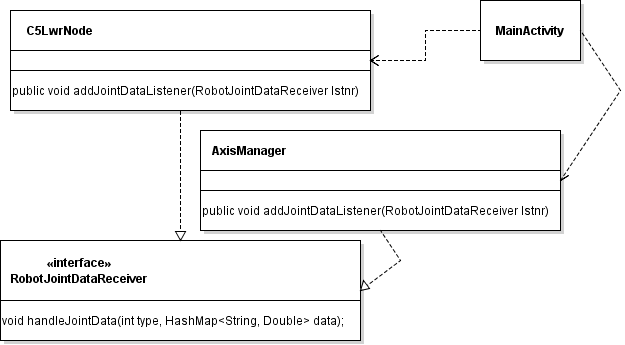
\includegraphics[width=\linewidth]{assets/chpt_concepts/sw/node_axismanager.png}
\end{wrapfigure}

\textit{AxisManager} and \textit{C5LwrNode} have to exchange joint data between each other in both directions. To accomplish this, both implement the \textit{RobotJointDataReceiver} interface (see Figure \ref{fig:conc:obs2}. The design here is relatively far away from the original observer pattern, as both classes do not know of each other. However, the common interface is used to notify each other about changes in the joint angles (either to send them to the robot or as they are received from it). The connection between both classes is made in the entry point of the Android application, \textit{MainActivity}. As \textit{MainActivity} manages the overall application set-up, it is the most suitable point to do so. If one or both of the classes were exchanged in later development, the only place that had to be changed to alter the connection would also be \textit{MainActivity}.

Aside from the original \textit{Observer} pattern described in \cite{Eilebrecht2013} multiple interfaces are described for observers to directly pass data to them. Following the conservative approach, observers would just be notified about changes, giving them the necessity to fetch them from the observed object on their own.

\subsection{Singleton}

As several classes exist of which only one instance is needed (and sensible to be created) within all of the application's functionality, the \textit{Singleton-Pattern} is used to ensure that only one instance exists. The singleton pattern is implemented by creating a private constructor which is called from a static method on the desired class. The created instance is saved into a static field and then returned on all subsequent calls. An example implementation of the pattern (as taken from \cite{Eilebrecht2013}) can be found in Listing \ref{lst:conc:obs}.

The \textit{Observer-Pattern} is implemented by the following classes:
\begin{itemize}
	\item \textit{AxisManager}, as it is important that all axis actions (and especially the safety interlock) are existent and performed just once over all of the application. Multiple instances of the \textit{AxisManager} may interfere with each other and thus cause unpredictable behaviour of the overall set-up.
	\item \textit{CartesianArmManager}, as it holds the current position of the arm in Cartesian coordinates. For the same reasons as with \textit{AxisManager}, having multiple instances (and states) of this class available in the application would not be sensible -- or even dangerous!
\end{itemize}

Only one instance exists during the runtime of other classes, too, like the \textit{C5LwrNode}. As for the above classes, having multiple instances available could cause unexpected and unwanted behaviour and thus it has to be ensured only one instance is created. However, with the node implementation ensuring this is not as easy as using the \textit{Singleton-Pattern}, because multiple parameters have to be passed to the class on creation. In this case, \textit{MainActivity}, as the main entry point for the application, takes care of the node's instance, passing it to all classes that need access to it. The same applies for all the user interface specific classes (mainly the \textit{Fragment} classes, offering the different tabbed views). Here, no singleton pattern can be used by Android's restrictions, so \textit{MainActivity} takes care of these, too.

\begin{minipage}{\linewidth}
\begin{lstlisting}[caption={Example implementation of the Observer-Pattern}, label=lst:conc:obs]
class Singleton {
	private static Singleton instance = null;

	public static Singleton getInstance() {
		if(instance == null) {
			instance = new Singleton();
		}
		
		return instance;
	}
	
	private Singleton() { }
}
\end{lstlisting}
\end{minipage}
